\documentclass{report}
%\usepackage{geometry}
%\geometry{top=0.5in} % Adjust the top margin as needed
\usepackage{graphicx}
% Packages for document formatting
\usepackage{titlesec}
\usepackage{tikz}
\usepackage{tocloft}
\usepackage{amsmath}
\usepackage{amssymb}
\usepackage{apacite}
%\usepackage{tocloft} % for customizing table of contents

% Command to create a separate list of figures
%\newcommand{\listfigurename}{List of Figures} % Customize the list of figures name
\usetikzlibrary{calc} 
\usepackage{lipsum} % For dummy text, remove this in your final document
\usepackage{natbib} % For citations and bibliography
\usepackage[top=0.5in,a4paper,margin=3cm]{geometry}
\begin{document}

\begin{titlepage}
    \begin{tikzpicture}[remember picture,overlay]
        \draw[line width=1pt]
        ($(current page.north west)+(1cm,-1cm)$) rectangle ($(current page.south east)+(-1cm,1cm)$);
    \end{tikzpicture}
    \centering
    \vspace*{1cm} % Vertical space before title
    
    % Title
    \Large{\textbf{Digital Content Security System Based on Image Steganography }}
    \vspace{1.5cm} % Vertical space after title
    
    % Author
     by\\

     Deena Faria\\
    Roll: 211020103

    \vspace{3cm} % Vertical space after author
    
    % Additional text
    A project submitted in partial fulfillment of the requirement for the degree of
    Master of Science in Computer Science and Engineering \par
    \vspace{1.5cm} % Vertical space after additional text
    
    % Image
    
\includegraphics[width=0.3\textwidth]{image1.jpeg}
    \par
    \vfill % Fill remaining space vertically
    Department of Computer Science and Engineering\\
    JATIYA KABI KAZI NAZRUL ISLAM UNIVERSITY, MYMENSINGH\\
    SUBMISSION YEAR, 2023
\end{titlepage}

\newpage
\newgeometry{top=1in}
\vspace{2cm}

The project titled “Digital Content Security System Based on Image Steganography” submitted by Deena Faria, Roll No.: 211020103, Session: MS 2020-21, has been accepted as satisfactory in partial fulfillment of the requirement for the degree of Master of Science in Computer Science and Engineering on 23/07/2023.

\vspace{2cm} % Adjust vertical space

\noindent
\textbf{\large BOARD OF EXAMINERS}\\

\noindent
\begin{minipage}[t]{0.8\textwidth}
    \begin{tabular}[t]{@{} l @{}}
        
        \quad Signature \\
        Dr. A.H.M Kamal \\
        Professor \\
        Dept. of CSE, JKKNIU \\
        \\
        \quad Signature \\
        Name of the Internal Member \\
        Designation \\
        Address \\
        \\
        \quad Signature \\
        Name of the Internal Member \\
        Designation \\
        Address \\
        \\
        \quad Signature \\
        Name of the External Member \\
        Designation \\
        Address \\
    \end{tabular}
\end{minipage}%
\hfill
\begin{minipage}[t]{0.4\textwidth}
    \begin{tabular}[t]{@{} l @{}}
        \vspace{2cm}
        Chairman \\
        \vspace{2cm}
        Member \\
        \vspace{2cm}
        Member \\
        \vspace{2cm}
        Member (External) \\
    \end{tabular}
\end{minipage}

\thispagestyle{empty}


\newpage
\begin{center}
    \textbf{\large CANDIDATE’S DECLARATION}
\end{center}
\vspace{1cm}
I declare that this project is my own work and has not been submitted in any other form for another degree or diploma at any university or other institute of tertiary education. Information derived from the published and unpublished work of others has been acknowledged in the text, and a list of references is given.

\vspace{2cm} % Adding vertical space

\noindent
\begin{minipage}[t]{0.6\textwidth}
    Date:
\end{minipage}%
\hfill
\begin{minipage}[t]{0.4\textwidth}
    \raggedleft
    \begin{tabular}[t]{@{} l @{}}
        \quad \quad Signature of the Candidate \\\\
        \quad Name of the Candidate: Deena Faria \\
    \end{tabular}
\end{minipage}
\thispagestyle{empty}
 
\newpage
\begin{center}
    \textbf{\large SUPERVISOR’S CONSENT FOR PROJECT SUBMISSION}
\end{center}

The undersigned have examined the report entitled “Digital Content Security System Based on Image Steganography” presented by Deena Faria for the course CSE-6000 and hereby certify that it is worthy of acceptance.

\vspace{1cm} % Adding vertical space

\noindent
\begin{minipage}[t]{0.6\textwidth}
    Date:
\end{minipage}%
\hfill
\begin{minipage}[t]{0.4\textwidth}
    \raggedleft
    \begin{tabular}[t]{@{} l @{}}
        Signature of the Supervisor \\\\
        ………………………… \\\\
        \qquad Dr. A.H.M Kamal \\\\
    \end{tabular}
\end{minipage}
\thispagestyle{empty}

\newpage
\begin{center}
    \textbf{\large DEDICATION}
\end{center}
\vspace{1cm}
I dedicate this project to my father.
\thispagestyle{empty}
\restoregeometry
% Abstract
\newgeometry{top=1in}
\section*{\centering Abstract}
\addcontentsline{toc}{section}{Abstract}

Steganography is the art and science of hiding data into some other cover media. Traditional LSB based techniques have some disadvantages and limitations like vulnerabilities and insecurities. The primary intention of  this research is to eliminating those limitations and developing an efficient technique that will utilize the full potential of the cover media and the transmission channel. We explored some refinement of traditional 24-bit RGB image based LSB steganography which will provide encryption as well as confidentiality by performing steganogarphy algorithm on the selected pixels. We also explored in the compression techniques for the cover images for the purpose of easy transferring the stego-images through the communication channels. I believe this project will be beneficiary for the systems that require excessive information hiding in significantly less pixels and also for slow networks to prevent network congestion. 
\pagenumbering{roman}

\newpage

% Acknowledgments
\section*{\centering Acknowledgments}
\addcontentsline{toc}{section}{Acknowledgments}
A project presents a tremendous opportunity for personal growth, learning, and exploration of new horizons. It serves as a catalyst for self-development, and I feel so grateful and privileged to be guided by such amazing individuals who direct me through in completion of this project\\ 
First and foremost, I would like to thank my honourable supervisor Professor Dr. A.H.M. Kamal, whose valuable insights and expertise have been pivotal in shaping the direction of this project. His unwavering support, patience and constructive feedback have been instrumental in driving this work forward.\\
I would like to extend my gratitude to the professor Dr. Md. Sujan Ali, Head of the Department, who has provided a conductive environment for learning and  research. I choose this moment to acknowledge his contribution gratefully.\\ 
I would also like to thank the Project Selection Committee for their efforts and favor towards me to get such an excellent opportunity. 
Lastly, so many tremendous people were there who shared invaluable information that guided me in the successful completion of this project.  

\restoregeometry
% Table of Contents
\newpage
\tableofcontents
\thispagestyle{empty} % Removes page number from table of contents

\newpage
\listoffigures
\thispagestyle{empty} % Removes page number from table of contents

\newpage
\pagenumbering{arabic}
% Sections
\chapter{Introduction}
\section{Background}
The word “steganography” comes from the greek “steganografia” which is the combination of the two words “steganos”; means covered and “graphia”; means writing. In literal sense, steganography means covered writing, that is, to hide any messages within a physical or virtual object. From the ancient time, steganography has been used for data confidentiality. Although, encryption ensures the security of the data for not to be disclosed to any unauthorized accesses, it itself is not enough to protect the confidential information from the attackers without raising any anticipation of the messsges’ containing secret data. For this reason, steganography was introduced as to not only encrypt the message but also to conceal it within another form of media.\\

Since the dawn of steganography, there has been a significant number of techniques developed for protecting the data from any unauthorized accesses or to prevent eavsdropping. \\


\begin{figure}[htbp]
  \centering
  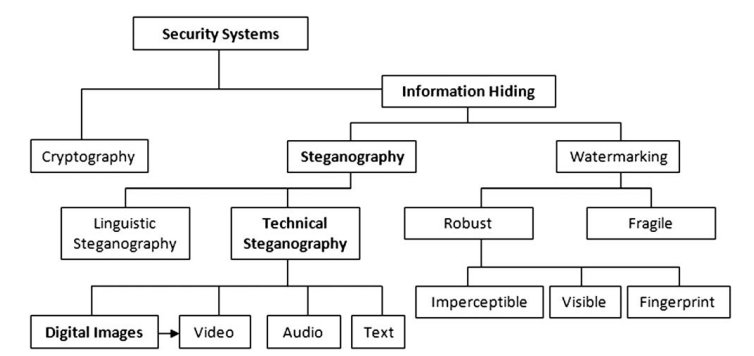
\includegraphics[width=0.7\textwidth, height=5.5cm]{image2.png} 
  \caption{The different embodiment disciplines of information hiding. The arrow indicates an extension and bold face indicates the focus of this study \cite{cheddad2010digital}}
  \label{fig:1}
\end{figure}

\vspace{0.5cm}
There has been different techniques for steganography, for example, image steganography, video steganography, audio steganography, and text steganography. Least Significant Bit (LSB) matching is the most popular technique in the field of image steganography.\\
In LSB steganography, secret data is hidden in the least significant bit of the cover image pixels. Since the least significant bit is altered, there is no significant amount of changes in the image.
\\
\begin{figure}[htbp]
  \centering
  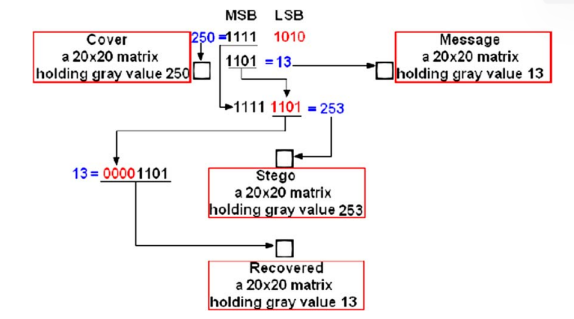
\includegraphics[width=0.7\textwidth, height=5.3cm]{image3.png} 
  \caption{Steganography in spatial domain. The effect of altering the LSBs up to the 4th bit plane.\cite{cheddad2010digital} }
  \label{fig:2}
\end{figure}
\\
\section{Motivation}
The principle motivation behind this project is to improving the existing systems in regards to the 24-bit color image based image steaganography. In the existing system, there could be some lsb bits left unaltered or unutilized if we fix the seed point for hiding the data and the data is larger than the number of the remaining bits in the lsbs of the image. In this case, we will define a new seed point for the data to be started embedding and utilize the full potential of the cover image to distribute the data uniformly across the image by our proposed technique. Besides this, we will also explore reducing the size of the generated stego image by some compression techniques for transferring the stego-images through low-bandwidth systems.
\section{Objective}
\begin{itemize}
    \item[1] Build a secure system using LSB steganography
    \item[2] Improve the existing system
    \item[3] Utilize the full cover image pixels to ensure concealing the whole message uniformly across the image.
    \item[4] Integrate encryption to protect unauthorized accesses 
    \item[5] Develop a technique to prevent steganalysis
    \item[6] Reducing the size of the stego image for storage and transmission purposes
\end{itemize}
\section{Outline}
The project report has five chapters in total. The first chapter describes the idea about our project “Digital Content Security System Based on Image Steganography”. The second chapter has given the overview of literature study and analysis. In the third chapter, there is a description of the methodology and design of the project. The fourth chapter shows the implementation i.e., output of the system. The fifth chapter includes future direction and discussion. Here we concluded the report. Then we provided references for the information that we used in this report.

\chapter{Literature Review and Analysis}

\section{Historical Background of Image Steganography} 
Image steganography has a rich history dating back to ancient civilizations when secret messages used to be concealed within paintings and drawings. In the digital age, the concept of steganography was reintroduced with the advent of digital media. Early works, such as prisoner’s problem by Simmons (1983) laid the foundation for modern steganographic techniques.\cite{bohme2010principles}\\

\section{Key Concepts and Techniques}
The most widely used steganographic technique is the Least Significant Bit (LSB) embedding. It involves replacing the least significant bit of selected pixels with the secret data. While LSB is simple and efficient, it suffers from low embedding capacity and vulnerability to detection. Jacob D. (2007) explains the LSB embedding technique and presents the evaluation results for 2,4,6 Least significant bits for a .png file and a .bmp file.\cite{neeta2006implementation}\\
Transform domain techniques, like Discrete Cosine Transform (DCT) and Discrete Wavelet Transform (DWT), offer increased embedding capacity and improved security. Fridrich et al. (2001) presented a steganographic algorithm based on DWT, achieving higher robustness against steganalysis.\cite{fridrich2001detecting}\\
\section{Recent Advancements}
Transform domain techniques, like Discrete Cosine Transform (DCT) and Discrete Wavelet Transform (DWT), offer increased embedding capacity and improved security. Different methods also were developed for steganalysis purposes. Fridrich et al. presented a reliable and accurate method for detecting least significant bit (LSB) nonsequential embedding in digital images.\cite{fridrich2001detecting} With the emergence of deep learning, steganographic methods have seen significant advancements. Meng et al. (2018) showed an approach which corresponds multiple steganographic algorithms to complex texture objects was presented for hiding secret message.\cite{meng2018fusion} Additionally, Meng et al. (2018) makes an overall conclusion on image information hiding based on deep learning.\cite{meng2018survey}\\
Hybrid techniques have also gained attention in recent years. Reddy(2012) proposed Secure Steganography using Hybrid Domain Technique (SSHDT), achieving better performance in terms of both capacity and robustness.\cite{reddy2012secure}\\
\section{Comparison of Methods}
Comparing the various steganographic methods, it becomes evident that LSB-based approaches are more susceptible to detection due to their simple nature. In contrast, transform domain techniques offer better security, but they may suffer from increased computational complexity. Deep learning methods show promising results in terms of security and capacity but require large datasets for training.
\section{Security and Vulnerabilities}
While image steganography provides a secure means of communication, it is not without vulnerabilities. Qian (2015), proposes a new paradigm for steganalysis to learn features automatically via deep learning models., can successfully detect steganographic content with high accuracy.\cite{qian2015deep} ,Therefore, the development of countermeasures to improve the resilience of steganography against detection remains an active research area.

\section{Applications}
Image steganography has applications in various domains. In the military and intelligence sectors, it enables covert communication and secure information exchange. Digital watermarking, as proposed by Cox et al. (2002), uses steganography to embed copyright information within images for copyright protection and content authentication.\cite{cox2007digital}
\section{Gaps and Future Directions}
Despite the progress was made in image steganography, there are still some challenges to be addressed. The limited capacity of existing methods hinders the secure transmission of large volumes of data. Moreover, the potential for adversarial attacks on deep learning-based steganography warrants further investigation.

\newpage
\chapter{Methodology}
\section{Existing System}
\subsection{Algorithm}
In this existing system, the secret message would be hidden in a cover bmp image. Firstly each character of secret message and each pixel of cover bmp image are converted into binary values. The user has to input stego-key as the password (stego-key is used to embed the secret message in a cover file). After inserting secret message into cover image file, the resulting stego-image is sent to the receiver through the desired communication channel. While defining the starting point of embedding LSB, the stego-key is firstly collected from the user. The summation of the ASCII value of each character of stegokey is calculated and then the average of those characters value is computed. While substituting the secret message into LSB of cover image, the first LSB position is chosen according to the calculated average value of input stego-key characters. Then the substitution processing will continue until the end of secret message. \\ 

\textbf{A.The embedding algorithm at the sender side }\\
Step (1) : Get the input cover image and secret message. \\
Step (2) : Accept the stego-key from the user and calculate average value of them. Step (3) : Convert each character of secret message and each LSB bit of cover image (R channel) from the position of average of stego-key. \\
Step (4) : Substitute the LSB bit of cover image (R channel) with binary values of secret message with respect to the starting point until the end of secret message. \\
Step (5) : Insert the end character value at the end of secret message. \\
Step (6) : Calculate the PSNR, SNR of original and resulting images. \\
Step (7) : Send a stego-image to the receiver. \\

\textbf{B. The extracting algorithm at the receiver side }
Step (1) : Get the input stego calculate average value \\
Step (2) : Load the stego-image that is sent from the sender. \\
Step (3) : Extract each of LSB bit from the stego image until to find out the end bit.\\
Step (4) : Reconstruct the collecting LSB bits from the stego-image. \\
Step (5) : Transform the LSB bits to correspondent characters\cite{aggarwal2019image}\\

\begin{figure}[htbp]
  \centering
  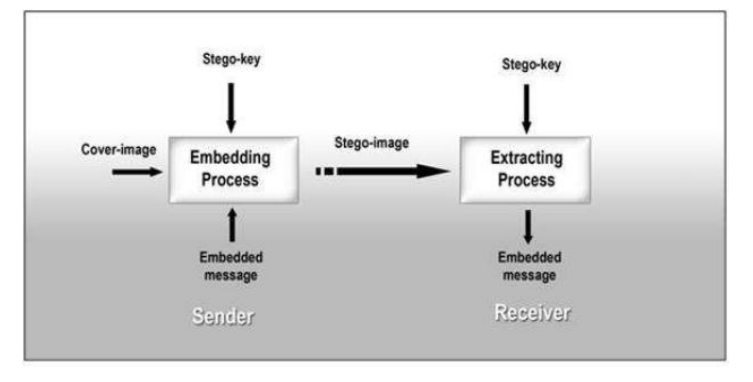
\includegraphics[width=0.7\textwidth, height=5cm]{image4.png} 
  \caption{The outline structure of the existing image steganography system\cite{aggarwal2019image} }
  \label{fig:3}
\end{figure}
\subsection{Limitations}
The above mentioned system has some disadvantages:\\
\begin{itemize}
    \item[1] There was a starting point described for the initial point but if the data bits exceed the image pixel boundaries, we can’t embed the full data in the cover image. 
    \item[2] Steganalysis of this system can be very easy as the algorithm used was very basic and thus, making it vulnerable to the attackers. 
    \item[3] No encryption mechanism was used to protect the data from third party access. 
\end{itemize}

\section{Proposed System}
To cope up with the above mentioned limitations, we developed a new technique.\\
\begin{figure}[htbp]
  \centering
  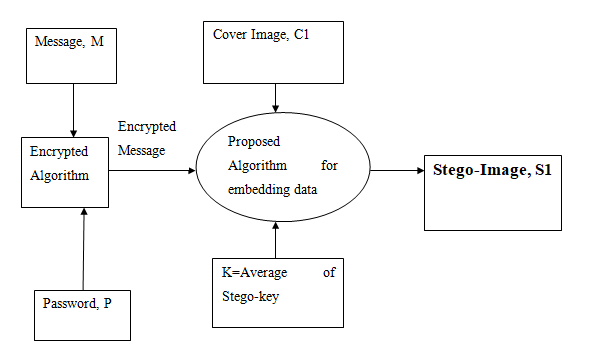
\includegraphics[width=0.7\textwidth, height=5cm]{Screenshot (363).png} 
  \caption{Simplified Block Diagram of the proposed technique}
  \label{fig:4}
\end{figure}
\subsection{Proposed Technique}

\begin{figure}[htbp]
  \centering
  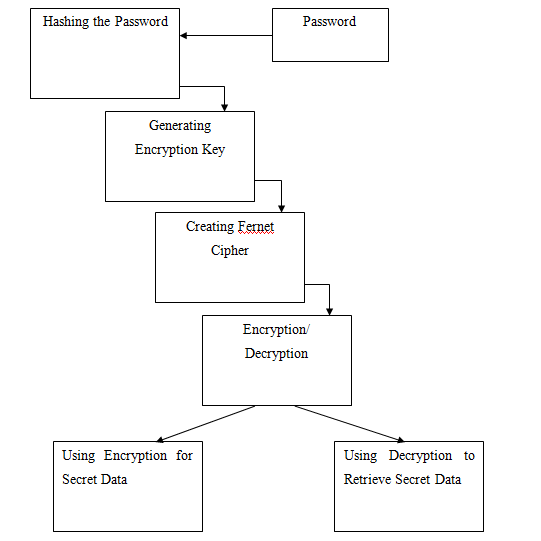
\includegraphics[width=0.7\textwidth, height=9cm]{image5.png} 
  \caption{Encryption/Decryption of the secret data }
  \label{fig:5}
\end{figure}

\subsubsection{Secret Message Encryption}
\begin{enumerate}
    \item \textbf{Hashing the Password:} \\
    The user provides a password as input to the function.
The function takes this password and applies a hash function (MD5) to it to generate a fixed-size hash value, represented as a hexadecimal string. Hashing is a one-way process, meaning one cannot reverse it to get the original password.
\item \textbf{Generating Encryption Key:}
The hashed password is then base64 encoded to ensure it is in a format suitable for encryption key generation.
This base64-encoded hash is used as the encryption key for the Fernet symmetric encryption.
\item \textbf{Creating Fernet Cipher:}
With the encryption key generated from the password, the function creates a Fernet cipher object. The Fernet cipher is specifically designed for symmetric encryption and decryption.
\item \textbf{Encryption or Decryption:}
The encrypt\_decrypt function takes three inputs: the string to be encrypted/decrypted, the password, and the mode. 
\item \textbf{Using Encryption for Secret Data:}
When the user chooses to encrypt secret data, the input text is passed to the encrypt\_decrypt function along with the provided password and the mode set to 'enc'. This way, the secret data is encrypted before embedding it into the image.
\item \textbf{Using Decryption to Retrieve Secret Data:}
When the user chooses to decrypt secret data from an encoded image, the function decode is called with the Stego key, image path, password, and mode set to 'dec'. This decrypts the embedded secret data using the provided password and returns the original data.

\end{enumerate}

\subsubsection{\textbf{\large {Secret Message Embedding Technique}}}
\subsubsection{Algorithm 1 for calculating stego-key}
\begin{enumerate}
    \item Calculate the size of the cover image C1, Encoding\_capacity = height*width
    \item Calculate the length of the  message M, LM
    \item Compute K1=avg(K), where K is the user provided stego key
    \item Calculate available pixels for encoding, Lp=Encoding\_capacity-K1
    \item If LM > LP, go to the next step.
    \item Define a new key, K2 = LP Mod LM
    \item Use K2 as the initial point for the secret message bit embedding position
    \item Else use K1 as the initial point
\end{enumerate}

\subsubsection{Algorithm 2 for uniformly distributing the message across the image}
\begin{enumerate}
    \item Calculate the stego key using algorithm 1
    \item Recalculate LP=Encoding\_capacity-  new stego key
    \item Compute pixel\_jump=LP/LM
    \item Compute LP=LC-K1
    \item Start modifying from the seed pixel (defined by the stego key) 
    \item Jump to the next pixel by an amount of pixel\_jump
    \item Continue step 5 until the end of the data or the image pixel.
\end{enumerate}

\textbf{Example:}
Let’s assume the height and the width of the image are 10 and 10 pixels respectively. Hence, the encoding capacity will be, Encoding-capacity=height*width=10*10. User provides a stego key as a string . Our algorithm will convert each character to its corresponding ASCII value and then calculate the average of these values which will be used as the initial stego key.  Let’s assume the value is 10.\\
Now, the available pixels, LP= Encoding-capacity-avg\\
Therefore, LP=100-10=90\\
Let’s assume the length of the message LM is, 5.\\
5 is smaller than 90, in this case we can retain the original stego key and calculate the values of the iterators accordingly.\\
I=width/avg=10\\
J=width-i*avg=0\\
Pixel\_jump=LP/LM =90/5=18\\
In this way, the entire message will be uniformly distributed across the whole image.

\begin{figure}[htbp]
  \centering
  
\includegraphics[width=0.7\textwidth, height=7cm]{Screenshot (355).png} 
  \caption{Initializing the seed pixel using stego-key}
  \label{fig:6}
\end{figure}

\begin{figure}[htbp]
  \centering
  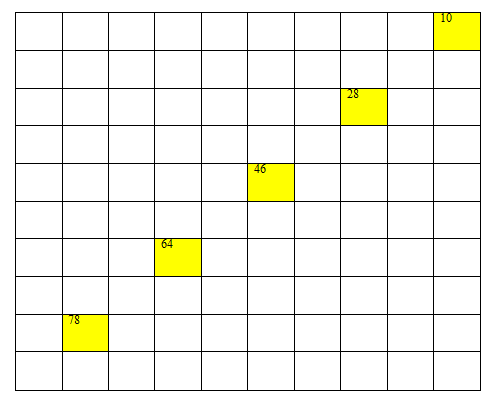
\includegraphics[width=0.7\textwidth, height=7cm]{Screenshot (357).png} 
  \caption{Uniform distribution of the data}
  \label{fig:7}
\end{figure}


\subsubsection{PNG image for storing purpose}
We used PNG image as the cover and the stego image

A PNG (Portable Network Graphics) image is a popular raster graphics file format used for storing images. PNG was created to replace the older and more limited GIF format while providing support for more colors and better transparency.\\
PNG images use lossless compression, which means that no image data is lost during compression. There are two main compression mechanisms used in PNG:
\\
\textbf{Deflate Compression:} PNG uses a compression algorithm called DEFLATE, which is a combination of LZ77 algorithm (Lempel-Ziv 1977) and Huffman coding. DEFLATE looks for repeated patterns in the image and replaces them with references, reducing the overall file size without losing any image data. It breaks down the image data into small chunks, analyzes the data for patterns, and then replaces repetitive sequences with references to previous occurrences.\\
\textbf{Filtering:} Before compressing the image data, PNG applies a filtering step. Filtering predicts the value of each pixel based on the values of neighboring pixels. The filter tries to reduce the amount of information needed to store the image by encoding the differences between pixel values rather than the absolute values. There are several filter types (None, Sub, Up, Average, Paeth) that PNG can use to predict pixel values, and the most suitable filter type is chosen for each row of pixels in the image.\\
PNG images offer the advantage of preserving image quality without sacrificing much on file size. However, compared to formats like JPEG, which use lossy compression, PNG files tend to be larger, especially for photographs or images with many colors. PNG is excellent for images with text, line art, logos, or images with transparent backgrounds because it maintains sharp edges and transparency without any loss of quality.

\textbf{Compression}\\
\textbf{Preprocessing:}\\
Before compression, the image data goes through a filtering step. This step predicts pixel values based on neighboring pixels to prepare the data for better compression.\\
\textbf{Filtering}\\
PNG uses various filtering algorithms (None, Sub, Up, Average, Paeth) to predict pixel values within each row of the image. This filtering step aims to reduce the amount of information required to store the image by encoding the differences between pixel values rather than absolute values.\\
\textbf{Deflate Compression:}\\
After filtering, the data undergoes DEFLATE compression. DEFLATE is a combination of LZ77 and Huffman coding. LZ77 identifies repeated patterns in the filtered image data and replaces them with references to reduce redundancy. Huffman coding assigns shorter codes to frequently occurring patterns, further reducing the overall file size.\\
\textbf{LZ77 Compression:}\\
In the LZ77 phase, the data is scanned, and repeated sequences of data (called "matches") are replaced by pointers back to the previous occurrence of the same sequence. This is achieved using a sliding window that stores recently encountered data.\\

\textbf{\large During decompression, the reverse process is performed:}\\
\textbf{Reverse Deflate Compression: } When a PNG image is opened or accessed, the compressed data is first decompressed using the DEFLATE algorithm. This reverses the compression process by reconstructing the original compressed data.\\
\textbf{Reverse Filtering: } After decompression, the filtered data is reversed to obtain the original pixel values. This involves applying the inverse of the filtering algorithm used during compression to predict the pixel values based on neighboring pixels.\\
\textbf{Reconstruction:} The reconstructed pixel values are used to recreate the image, maintaining the original quality and transparency information.\\

\newpage
\chapter{Implementation}
\section{Overview}
Implementation phase is the operational phase of the system. In this phase, the program code for the development is written following the system requirements and specification from the design stage. It is a crucial step in constructing the new system as it brings the system to life. The previous phases lay the groundworks and blueprints for the system development; The Implementation phase is where these plans are put into action to create the final product. This stage ensures that the system functions as intended, meeting all the specified requirements and objectives outlined in the earlier phases.

\section{System Architecture}
\begin{figure}[htbp]
  \centering
  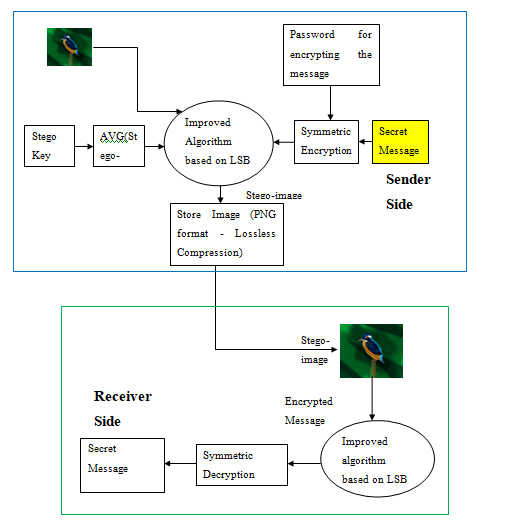
\includegraphics[width=0.7\textwidth, height=8cm]{Screenshot (359).png} 
  \caption{Architectural design for the proposed system }
  \label{fig:6}
\end{figure}
We used a PNG image and a dummy text to test our system. A stego key had been taken from the user which was a "string literal". A function calculated the average of the ASCII values of the letters contained in the string. Then, we calculated the available pixels by subtracting the average value from the encoding capacity of the image. We performed some checking to test if the data could fit within the available image. And, lastly we applied our improved algorithm to embed the data uniformly across the image. 

\newpage
\section{Output of the System}
\begin{figure}[htbp]
  \centering
  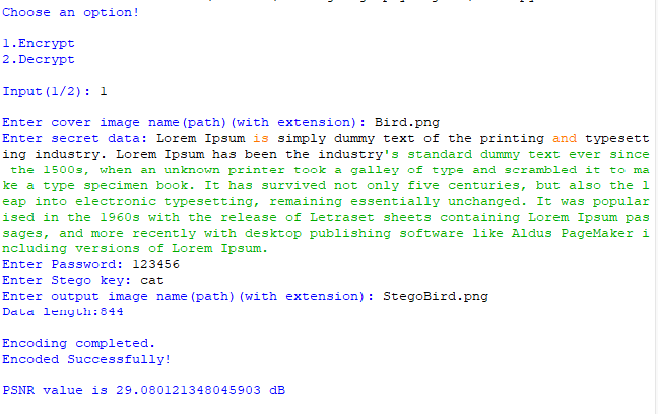
\includegraphics[width=0.7\textwidth, height=6cm]{Screenshot (360).png} 
  \caption{Sender Side }
  \label{fig:7}
\end{figure}

\begin{figure}[htbp]
  \centering
  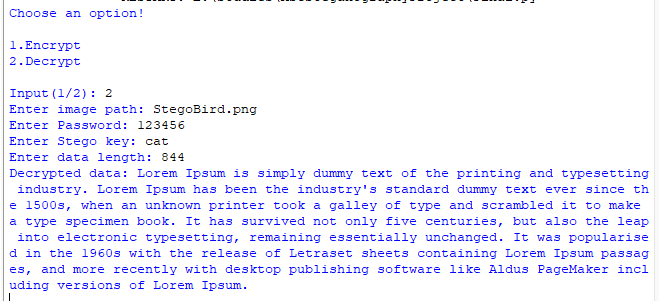
\includegraphics[width=0.7\textwidth, height=5cm]{Screenshot (361).png} 
  \caption{Receiver Side }
  \label{fig:8}
\end{figure}

\section{Result and Analysis}
\subsection{Result}
The output we provided is the progress that we have made so far. Users have to provide a cover image, a secret data, a password, and a stego key. The system encrypt the data using fernet encryption using the password and the stego key is used to determine the initial point on the cover image for embedding.

\subsection{Analysis}
For now, we have tested the system with relatively simple input data. It worked successfully. The PSNR value is low (29 dB, approximately), but we will work on this later.

\subsubsection{PSNR}
PSNR stands for Peak Signal-to-Noise Ratio. It is a widely used metric to measure the quality of an image or video signal after compression or data embedding. PSNR is commonly used in image processing, video encoding, and steganography to assess how much an image has been distorted compared to the original, uncompressed or unmodified version.\\
The PSNR value is expressed in decibels (dB) and provides a numerical indication of the image quality. A higher PSNR value generally indicates better image quality, whereas a lower value indicates more significant distortion or loss of information.\\
Here's how PSNR is calculated:\\
Mean Squared Error (MSE): The first step in calculating PSNR is to compute the Mean Squared Error between the original and compressed (or modified) images. MSE represents the average of the squared differences between corresponding pixels in the two images. It is calculated using the following formula:\\
\begin{equation*}
    \text{MSE} = \frac{1}{\text{Total Number of Pixels}} \sum_{i=1}^{N} (\text{Original Pixel}_i - \text{Compressed Pixel}_i)^2
\end{equation*}
\\
Maximum Pixel Value (MaxPixel): The maximum pixel value represents the highest possible intensity value that a pixel can take in the image. For example, for an 8-bit grayscale image, the maximum pixel value is 255.\\
PSNR Calculation: Once the MSE and MaxPixel values are determined, the PSNR is calculated using the following formula:
\begin{equation*}
    \text{PSNR} = 20 \cdot \log_{10}\left(\frac{\text{MaxPixel}}{\sqrt{\text{MSE}}}\right)
\end{equation*}

The logarithmic scale is used to provide a more intuitive representation of the image quality.\\
Interpretation of PSNR:\\
A PSNR value of 30 dB or higher is generally considered to indicate excellent image quality, meaning that the compression or modification had a minimal impact on the visual fidelity of the image.\\
A PSNR value between 20 dB and 30 dB indicates good image quality, although there might be some noticeable loss of detail.
PSNR values below 20 dB indicate significant loss of image quality, and the image may appear visibly distorted to the human eye.\\

\newpage
\newgeometry{top=0.5in}
\chapter{Conclusion}
The provided system showcases a simple implementation of image encryption and steganography using the Fernet symmetric encryption and LSB steganography techniques. The system allows users to encrypt a secret message using a password and embed it within an image, creating a stego image. The stego image appears visually similar to the original cover image, and the embedded secret data remains hidden to the bare human eyes.\\\\
The system successfully achieved its primary objectives, which are encryption, data hiding, and image retrieval. The use of symmetric encryption with the Fernet cipher provides a simple yet effective way to secure the secret data before embedding it into the image. The added option to use a password enhances the security of the system, making it more challenging for unauthorized users to access the concealed data.\\\\
The LSB steganography technique, allows for the hiding of data within the least significant bits of the image pixels. We successfully embedded the data uniformly across the image according to our proposed algorithm. \\\\
We also calculated the Peak Signal-to-Noise Ratio (PSNR) to assess the image quality degradation caused by data embedding. The achieved PSNR value is a reasonable indicator of the image fidelity, showing that the steganography process resulted in minimal visible distortion to the cover image.\\\\
The system provides a practical demonstration of  image encryption and steganography, serving as a tool to understand the underlying concepts. We learned about symmetric encryption, steganography, PSNR calculation, and the importance of secure password management. For practical use in real-world scenarios, we will work on the system's security and capabilities to be further enhanced and scrutinized in the future.


% References
\bibliographystyle{apacite}
\section*{\bibliography{references}}
\addcontentsline{toc}{section}{References}
\end{document}
